\documentclass[12pt,a4paper,oneside]{report}

\usepackage[utf8]{inputenc}
\usepackage[T1]{fontenc}
\usepackage{babel}
\babelprovide[import,main]{spanish}
\addto\captionsspanish{\renewcommand{\tablename}{Tabla}}
\usepackage{geometry}
\usepackage{graphicx}
\usepackage{booktabs}
\usepackage{longtable}
\usepackage{array}
\usepackage{xcolor}
\usepackage{float}
\usepackage{listings}
\usepackage{needspace}
\usepackage{pgfplots}
\usepackage{hyperref}
\pgfplotsset{compat=1.18}
\setlength{\emergencystretch}{3em}

\renewcommand{\lstlistingname}{Listado}
\lstdefinestyle{pseudocodigo}{
  basicstyle=\ttfamily\small,
  frame=single,
  breaklines=true,
  columns=fullflexible,
  keepspaces=true,
  showstringspaces=false,
  xleftmargin=0.5em,
  xrightmargin=0.5em
}
\lstdefinestyle{codigoC}{
  language=C,
  basicstyle=\ttfamily\footnotesize,
  keywordstyle=\color{blue!60!black},
  commentstyle=\color{green!40!black},
  stringstyle=\color{red!50!black},
  frame=single,
  breaklines=true,
  columns=fullflexible,
  keepspaces=true,
  showstringspaces=false,
  numbers=left,
  numberstyle=\tiny\color{gray},
  xleftmargin=1.5em
}
\lstdefinestyle{comandos}{
  language=bash,
  basicstyle=\ttfamily\footnotesize,
  keywordstyle=\color{blue!60!black},
  commentstyle=\color{green!40!black},
  frame=single,
  breaklines=true,
  columns=fullflexible,
  keepspaces=true,
  showstringspaces=false,
  xleftmargin=0.5em,
  xrightmargin=0.5em
}

\geometry{top=2.5cm,bottom=2.5cm,left=3cm,right=2.5cm}
\hypersetup{
  colorlinks=true,
  linkcolor=black,
  citecolor=black,
  urlcolor=blue,
  pdftitle={Diseño y evaluación de anti-bunny-virus}
}

\begin{document}

\pagenumbering{roman}

\tableofcontents

\clearpage
\pagenumbering{arabic}
\chapter{Introducción}

\section{Problema y propósito del proyecto}

El agotamiento de procesos, CPU, memoria o almacenamiento puede degradar un
sistema Linux hasta impedir su operación y recuperación. Este riesgo puede
originarse mediante proliferación recursiva de procesos, incluso desde
mecanismos legítimos como el aislamiento por sitio de un navegador
\cite{gierlings2023isolated}. El aislamiento de recursos, por su parte, puede
preservar la interactividad frente a cargas extremas de procesos y memoria
\cite{yang2008redline}.

En este proyecto, \emph{bunny virus} designa un comportamiento sostenido de
agotamiento: creación acelerada de procesos, aumento de memoria o crecimiento
continuo de un archivo. Los cambios de tamaño y otros metadatos permiten
observar actividad sospechosa en almacenamiento \cite{pennington2003storage},
pero una monitorización frecuente también introduce un coste dependiente de la
carga \cite{patil2004i3fs}. Por ello, \emph{anti-bunny-virus} obtiene muestras
de procesos y recursos desde \texttt{/proc}, vigila un directorio configurado y
evalúa tasas temporales y persistencia. Cada alerta conserva su evidencia y la
contención solo puede aplicarse, en laboratorio, a un grupo atribuible y
autorizado.

La pregunta de investigación es: ¿un monitor en C para Linux basado en tasas
temporales, persistencia y correlación puede detectar tempranamente escenarios
controlados de agotamiento y contener de forma segura el grupo responsable? La
evaluación se limita a los simuladores, configuración y máquinas virtuales
descritos; no pretende demostrar protección general contra malware.

\section{Hipótesis}

Se plantea que las tasas temporales y la persistencia permitirán detectar los
tres simuladores antes de sus límites configurados. Asimismo, la validación de
identidad y autorización debería permitir contener únicamente el grupo de
laboratorio, sin alertas críticas durante la línea base. La hipótesis se
evaluará mediante latencia de alerta y contención, recursos consumidos, falsos
positivos, recuperación y sobrecarga del monitor, y sus conclusiones se
restringirán al entorno experimental.

\clearpage

\section{Objetivos}

\subsection{Objetivo general}

Diseñar, implementar y evaluar un monitor en C para Linux capaz de detectar
comportamientos controlados de agotamiento de procesos, memoria y almacenamiento,
y de aplicar una respuesta trazable y segura sobre un grupo autorizado en un
entorno de laboratorio.

\subsection{Objetivos específicos}

\begin{enumerate}
  \item Recolectar desde Linux la relación entre procesos, el consumo de CPU y
  memoria, y el crecimiento de archivos, incluyendo la atribución del archivo a
  un proceso cuando exista evidencia suficiente.

  \item Detectar anomalías sostenidas mediante tasas temporales, umbrales y
  persistencia, y registrar para cada alerta las métricas que originaron la
  decisión.

  \item Implementar una política de contención de laboratorio que valide la
  identidad y autorización del proceso o grupo antes de enviar señales, y que
  rechace acciones sobre objetivos no autorizados.

  \item Comparar experimentalmente los escenarios sin protección, con detección
  y con contención, midiendo latencia de alerta, consumo de recursos, falsos
  positivos, recuperación y sobrecarga del monitor.
\end{enumerate}

\chapter{Sistema anti-bunny-virus}

\section{Arquitectura y funcionamiento general}

\emph{Anti-bunny-virus} es un monitor de espacio de usuario. Cada 0,25 s obtiene
procesos y recursos desde \texttt{/proc}, mide un directorio, evalúa reglas y
registra o contiene la amenaza. Al iniciar configura el log, el modo de respuesta
y la autorización del laboratorio. Usa arreglos estáticos para un máximo de
8192 procesos y recursos, 1024 archivos y 256 alertas por ciclo.

\paragraph{Organización del código.}
El repositorio separa recolectores (\texttt{monitor\_procesos},
\texttt{monitor\_recursos}, \texttt{monitor\_archivos}), el motor
(\texttt{motor\_deteccion}), la respuesta (\texttt{respuesta}) y el ciclo
principal (\texttt{main.c}). La versión integrada desde \texttt{main} mantiene
el mismo comportamiento evaluable, pero documenta en comentarios el propósito de
cada función pública y de los pasos críticos (historial por
\texttt{starttime}, persistencia, atribución y contención). Los simuladores en
\texttt{simuladores/} incluyen la misma documentación breve sobre la carga que
generan.

\begin{figure}[htbp]
  \centering
  \fbox{\parbox{0.78\textwidth}{\centering
    Recolección de procesos, CPU/RSS y archivos}}
  \par\smallskip$\Downarrow$\par\smallskip
  \fbox{\parbox{0.78\textwidth}{\centering
    Historial por PID--\texttt{starttime} y por ruta}}
  \par\smallskip$\Downarrow$\par\smallskip
  \fbox{\parbox{0.78\textwidth}{\centering
    Tasas temporales, umbrales y persistencia}}
  \par\smallskip$\Downarrow$\par\smallskip
  \fbox{\parbox{0.78\textwidth}{\centering
    Alerta con severidad, identidad y evidencia}}
  \par\smallskip$\Downarrow$\par\smallskip
  \fbox{\parbox{0.78\textwidth}{\centering
    Registro o contención del grupo autorizado}}
  \caption{Flujo principal del sistema anti-bunny-virus.}
  \label{fig:flujo-sistema}
\end{figure}

El Listado~\ref{alg:ciclo-principal} resume \texttt{main.c}. Todas las alertas
se registran; las señales solo se envían bajo la política de la
Sección~\ref{sec:deteccion-respuesta}.

\Needspace{18\baselineskip}
\begin{lstlisting}[style=pseudocodigo,caption={Funcionamiento general de anti-bunny-virus.},label={alg:ciclo-principal}]
configurar log, modo y autorizacion de laboratorio
instalar manejador de SIGINT
inicializar historiales de procesos, recursos y archivos

mientras la ejecucion siga activa:
    procesos <- recolectar procesos desde /proc
    recursos <- recolectar CPU y RSS desde /proc
    archivos <- medir archivos del directorio vigilado

    comparar cada muestra con su historial
    calcular hijos nuevos y CPU
    calcular crecimiento_RAM en MB/s
    calcular crecimiento_archivo en MB/s

    si existen archivos:
        mayor <- archivo con mayor crecimiento_archivo
        si crecimiento_archivo(mayor) > 0:
            atribuir mayor a un proceso, si es posible

    alertas <- detectar(procesos, recursos, archivos)
    registrar y responder(alertas, modo)
    actualizar historiales
    esperar 0.25 segundos
\end{lstlisting}

\section{Monitorización y extracción de métricas}

\paragraph{Procesos.}

\texttt{monitor\_procesos} recorre los PID de \texttt{/proc} y obtiene los datos
de la Tabla~\ref{tab:campos-proceso}. Si un proceso termina durante la lectura,
descarta esa muestra.

\begin{table}[H]
  \centering
  \small
  \caption{Datos recolectados para cada proceso.}
  \label{tab:campos-proceso}
  \begin{tabular}{p{0.22\textwidth}p{0.31\textwidth}p{0.36\textwidth}}
    \toprule
    \textbf{Dato} & \textbf{Fuente} & \textbf{Uso} \\
    \midrule
    PID, PPID y PGID & \texttt{/proc/[pid]/stat} & Identidad, relación padre--hijo y grupo de contención. \\
    Tiempo de inicio & \texttt{/proc/[pid]/stat} & Diferencia procesos que reutilizan el mismo PID. \\
    UID y usuario & Metadatos de \texttt{/proc/[pid]} & Verifica el propietario autorizado. \\
    Nombre y ejecutable & \texttt{stat} y \texttt{exe} & Describe la evidencia de la alerta. \\
    Hijos & Comparación de PPID & Detecta proliferación por proceso padre. \\
    \bottomrule
  \end{tabular}
\end{table}

El módulo cuenta los hijos por PPID. El historial identifica cada proceso por
PID y tiempo de inicio para evitar confusiones si el PID se reutiliza. Los hijos
nuevos y su tasa son

\begin{equation}
  H_{\mathrm{nuevos}}(p,t)=\max(0,H(p,t)-H(p,t-1)),
\end{equation}

\begin{equation}
  R_H(p,t)=\frac{H_{\mathrm{nuevos}}(p,t)}{\Delta t},
\end{equation}

donde $\Delta t$ proviene de un reloj monotónico. El historial se actualiza al
final de cada ciclo.

\paragraph{CPU y memoria.}

\texttt{monitor\_recursos} lee los ticks de CPU de
\texttt{/proc/[pid]/stat} y la memoria residente \texttt{VmRSS} de
\texttt{/proc/[pid]/status}. También identifica el historial mediante PID y
tiempo de inicio.

Sea $C_t$ la suma de ticks de CPU en la muestra actual, $f$ la frecuencia de
ticks del sistema y $M_t$ la memoria residente en MB. Las métricas implementadas
son

\begin{equation}
  \mathrm{CPU}(t)=\frac{(C_t-C_{t-1})/f}{\Delta t}\times 100,
\end{equation}

\begin{equation}
  \Delta\mathrm{RSS}(t)=\frac{M_t-M_{t-1}}{\Delta t}.
\end{equation}

La primera muestra produce tasas iguales a cero. La CPU calculada corresponde
al proceso durante el intervalo, no a la carga global de la máquina virtual.

\paragraph{Archivos y atribución.}

El monitor recorre \path{/tmp/anti_bunny_demo} y conserva el tamaño de cada
ruta. Si $S_t$ es el tamaño actual e $I$ el intervalo, calcula

\begin{equation}
  R_A(t)=\frac{\max(0,S_t-S_{t-1})}{1024^2 I}\quad\mathrm{MB/s}.
\end{equation}

Una disminución o una ruta nueva produce tasa cero. En cada ciclo solo se intenta
atribuir el archivo de mayor crecimiento.

La atribución compara la ruta con los enlaces de \texttt{/proc/[pid]/fd}, como
muestra el Listado~\ref{lst:atribucion}. Conserva el primer PID y PGID
coincidente. Sin coincidencia puede existir alerta, pero no contención.

\begin{lstlisting}[style=codigoC,caption={Comparación usada para atribuir un archivo abierto.},label={lst:atribucion}]
longitud = readlink(ruta_fd, enlace, sizeof(enlace) - 1);
if (longitud < 0) continue;
enlace[longitud] = '\0';
if (strcmp(enlace, archivo->ruta) == 0) {
    archivo->pid_escritor = procesos[i].pid;
    archivo->pgid_escritor = procesos[i].pgid;
    archivo->atribuido = 1;
    closedir(fds);
    return;
}
\end{lstlisting}

La atribución solo identifica archivos abiertos durante el sondeo; no constituye
evidencia forense de una escritura concreta.

\section{Detección y respuesta}
\label{sec:deteccion-respuesta}

\paragraph{Motor de detección.}

El motor identifica cada estado por tipo, PID y tiempo de inicio. Cuenta ciclos
anómalos y solo emite otra alerta si aumenta la severidad; al normalizarse,
reinicia el estado. La Tabla~\ref{tab:umbrales} contiene los umbrales.

\begin{table}[H]
  \centering
  \small
  \caption{Parámetros de detección configurados.}
  \label{tab:umbrales}
  \begin{tabular}{p{0.43\textwidth}p{0.18\textwidth}p{0.24\textwidth}}
    \toprule
    \textbf{Parámetro} & \textbf{Valor} & \textbf{Aplicación} \\
    \midrule
    Intervalo de monitorización & 0,25 s & Todos los recolectores. \\
    Hijos por proceso & 20 & Regla de proliferación. \\
    Hijos totales o nuevos por ventana & 8 & Inicio temprano de proliferación. \\
    Persistencia crítica & 2 ciclos & Procesos, recursos y archivos. \\
    Memoria residente & 256 MB & Regla de recursos. \\
    Crecimiento de RSS & 32 MB/s & Regla de recursos y correlación. \\
    CPU del proceso & 80\% & Regla de recursos y correlación. \\
    Crecimiento de archivo & 5 MB/s & Regla de archivos. \\
    Gracia de terminación & 2 s & Escalamiento de señales. \\
    \bottomrule
  \end{tabular}
\end{table}

Los dos umbrales expresados en MB/s miden objetos distintos:
\emph{crecimiento de RSS} es el aumento de RAM ocupada por un proceso, mientras
que \emph{crecimiento de archivo} es el aumento de una ruta en disco.

La proliferación genera una alerta sospechosa y pasa a crítica y accionable tras
dos ciclos o al alcanzar 40 hijos. CPU, RSS y archivos solo generan alertas no
accionables. Una alerta de archivo puede ser crítica si su escritor también
supera CPU o crecimiento de RSS. Por tanto, solo la proliferación puede activar
contención.

El Listado~\ref{lst:regla-procesos} muestra la regla de proliferación en C.

\Needspace{13\baselineskip}
\begin{lstlisting}[style=codigoC,caption={Clasificación de la proliferación de procesos.},label={lst:regla-procesos}]
int activo = procesos[i].hijos >= max_hijos ||
             procesos[i].hijos >= max_hijos_nuevos ||
             procesos[i].hijos_nuevos >= max_hijos_nuevos;

int critica = ciclos >= ciclos_persistencia ||
              procesos[i].hijos >= max_hijos * 2;

agregar(alertas_out, &total, max_alertas,
        procesos[i].pid, procesos[i].pgid,
        procesos[i].starttime, procesos[i].uid,
        critica, critica ? "critica" : "sospechosa",
        "procesos",
        critica ? "Proliferacion de procesos persistente"
                : "Proliferacion de procesos observada",
        evidencia);
\end{lstlisting}

\Needspace{32\baselineskip}
El Listado~\ref{alg:deteccion} resume las tres reglas con nombres explícitos
para RAM y archivos.

\begin{lstlisting}[style=pseudocodigo,caption={Motor de detección y clasificación.},label={alg:deteccion}]
para cada proceso p:
    si hijos_totales(p) >= 8 o hijos_nuevos(p) >= 8:
        aumentar ciclos_anomalos(p)
        si ciclos_anomalos(p) >= 2 o hijos_totales(p) >= 40:
            emitir alerta CRITICA y ACCIONABLE
        si no:
            emitir alerta SOSPECHOSA y NO ACCIONABLE
    si no:
        reiniciar ciclos_anomalos(p)

para cada recurso r:
    RAM_actual <- RSS(r) en MB
    crecimiento_RAM <- cambio de RSS por segundo
    si CPU(r) > 80 o RAM_actual > 256
       o crecimiento_RAM > 32 MB/s:
        aumentar ciclos_anomalos(r)
        si ciclos_anomalos(r) >= 2:
            emitir alerta SOSPECHOSA y NO ACCIONABLE
    si no:
        reiniciar ciclos_anomalos(r)

para cada archivo a:
    crecimiento_archivo <- cambio de tamano por segundo
    si crecimiento_archivo > 5 MB/s:
        aumentar ciclos_anomalos(a)
        si ciclos_anomalos(a) >= 2:
            si el escritor supera CPU o crecimiento_RAM:
                emitir alerta CRITICA y NO ACCIONABLE
            si no:
                emitir alerta SOSPECHOSA y NO ACCIONABLE
    si no:
        reiniciar ciclos_anomalos(a)
\end{lstlisting}

\paragraph{Registro y contención.}

Cada alerta se escribe en la salida estándar y en \texttt{logs/eventos.log} con
una línea \texttt{WARNING} que incluye fecha, severidad, tipo, PID, PGID,
\texttt{starttime}, descripción, evidencia y modo. Las acciones de contención o
denegación se registran como líneas \texttt{INFO} o \texttt{ERROR} con el mismo
formato de campos clave--valor.

El modo predeterminado \texttt{alerta} solo registra. En
\texttt{terminar\_lab}, la alerta debe ser crítica y accionable; PID y PGID deben
ser mayores que uno; y PGID, UID y tiempo de inicio deben coincidir con
\texttt{/proc} y la autorización. El Listado~\ref{lst:identidad} muestra la
revalidación.

\begin{lstlisting}[style=codigoC,caption={Revalidación de la identidad antes de contener (\texttt{respuesta.c}).},label={lst:identidad}]
if (stat(ruta, &datos) != 0) return 0;
pgid_actual = getpgid(a->pid);

return starttime_actual == a->starttime &&
       pgid_actual == a->pgid &&
       datos.st_uid == uid_laboratorio;
\end{lstlisting}

Tras autorizar, envía \texttt{SIGTERM} al PGID y espera dos segundos. Si el grupo
sigue activo y supera una nueva validación, envía \texttt{SIGKILL}. Toda acción
o denegación queda registrada.

El Listado~\ref{alg:contencion} resume esta secuencia.

\Needspace{16\baselineskip}
\begin{lstlisting}[style=pseudocodigo,caption={Contención gradual del grupo autorizado.},label={alg:contencion}]
para cada alerta:
    escribir alerta y evidencia en el log

    si modo != terminar_lab:
        continuar
    si alerta no es critica o no es accionable:
        registrar denegacion y continuar
    si PID, PGID, UID o starttime no coinciden:
        registrar denegacion y continuar

    enviar SIGTERM al grupo autorizado
    esperar 2 segundos
    comprobar que el grupo siga activo
    revalidar PGID, UID y starttime
    si continua activo y autorizado:
        enviar SIGKILL al mismo grupo
\end{lstlisting}

\Needspace{22\baselineskip}
\section{Simuladores y ejecución controlada}

\paragraph{Configuración y ejecución.}

Los umbrales están en \texttt{src/config.h}. El modo y la ruta del log admiten
variables de entorno. El Listado~\ref{lst:ejecucion-local} muestra la ejecución
local.

\begin{lstlisting}[style=comandos,caption={Compilación y ejecución local en modo de alerta.},label={lst:ejecucion-local}]
make check

# Terminal 1: solo registra; no envia senales
ANTI_BUNNY_MODE=alerta ./anti-bunny-virus

# Terminal 2: ejecutar un solo simulador por corrida
./simuladores/simulador_fork_bomb
./simuladores/simulador_memoria
./simuladores/simulador_archivo
\end{lstlisting}

\paragraph{Simuladores incluidos.}

Debe ejecutarse un simulador por corrida y solo dentro de la máquina virtual. La
Tabla~\ref{tab:simuladores} resume la carga y el resultado esperado.

\begin{table}[H]
  \centering
  \small
  \caption{Simuladores controlados del repositorio.}
  \label{tab:simuladores}
  \begin{tabular}{p{0.17\textwidth}p{0.32\textwidth}p{0.39\textwidth}}
    \toprule
    \textbf{Simulador} & \textbf{Carga ejecutada} & \textbf{Resultado esperado} \\
    \midrule
    Procesos & Hasta 64 procesos; ocho hijos por proceso; permanencia de 5 s. & Alerta de proliferación; crítica y accionable al persistir. \\
    Memoria & Diez asignaciones de 32 MB; máximo nominal de 320 MB. & Alerta sospechosa por RSS o crecimiento de memoria. \\
    Archivo & Ocho escrituras de 2 MB cada 0,2 s; total de 16 MB. & Alerta por crecimiento; incluye ruta y escritor si se atribuye. \\
    \bottomrule
  \end{tabular}
\end{table}

Solo el simulador de procesos puede activar contención. systemd lo aísla con
\texttt{setsid}, publica su PGID y limita el servicio a 256 PID. Tras instalar
\texttt{deploy/}, se ejecuta como indica el
Listado~\ref{lst:ejecucion-protegida}.

\begin{lstlisting}[style=comandos,caption={Ejecución del escenario protegido con systemd.},label={lst:ejecucion-protegida}]
sudo systemctl start anti-bunny-virus.service
sudo systemctl start anti-bunny-attack.service
sudo journalctl -u anti-bunny-virus.service -f
\end{lstlisting}

Memoria y archivo solo validan detección; no solicitan terminación. El simulador
de archivo escribe \path{/tmp/anti_bunny_demo/archivo_crecimiento_demo.bin}.
Los tres simuladores son acotados.

\chapter{Metodología de evaluación}

\section{Entorno y escenarios}

La evaluación se planteó como un experimento controlado con dos máquinas
virtuales (VM) Linux aisladas en Google Cloud. En la VM de control se ejecutó
la carga sin el monitor; en la VM protegida se mantuvo activo Anti-Bunny Virus.
La unidad experimental es una corrida completa, desde la línea base hasta la
recuperación o finalización de la carga. Para una comparación directa, ambas
condiciones deben usar recursos equivalentes; las capturas disponibles no
permiten comprobar esa equivalencia en todos los parámetros.

\begin{table}[H]
  \centering
  \caption{Configuración documentada para la evaluación.}
  \label{tab:entorno-evaluacion}
  \small
  \begin{tabular}{p{0.28\textwidth}p{0.62\textwidth}}
    \toprule
    Elemento & Configuración \\
    \midrule
    Plataforma & Google Cloud, región \texttt{us-central1} (Iowa). \\
    VM de control & \texttt{vm1-sacrificable}: 2 vCPU, 4 GB de RAM y disco persistente de 10 GB en la pantalla de configuración. \\
    VM protegida & \texttt{vm2-protegida}: arquitectura x86-64 y disco de origen de 25 GB. \\
    Snapshot protegido & \texttt{snap-limpio}, instantánea estándar de 937,58 MB. \\
    Recursos en terminal & Las capturas de ejecución muestran 1,9 GiB utilizables y 0 B de \emph{swap}. \\
    Versión del software & Código de \texttt{main} (commit \texttt{a771cbc}), integrado en la rama del informe; verificado con \texttt{make check}. \\
    Muestreo del monitor & Un ciclo cada 0,25 s. \\
    Condición de control & Monitor inactivo y ejecución de la carga de procesos. \\
    Condición protegida & Monitor activo; modo \texttt{alerta} en la evidencia JSON. \\
    Identidad observada & Usuario \texttt{antibunny-test} y PGID 12480 en el JSON. \\
    Freno independiente & \texttt{PIDsMax=256} en la unidad protegida de \texttt{systemd}. \\
    Datos aún no consignados & Distribución, kernel, vCPU/RAM de la VM protegida y snapshot de la VM de control. \\
    \bottomrule
  \end{tabular}
\end{table}

\begin{figure}[H]
  \centering
  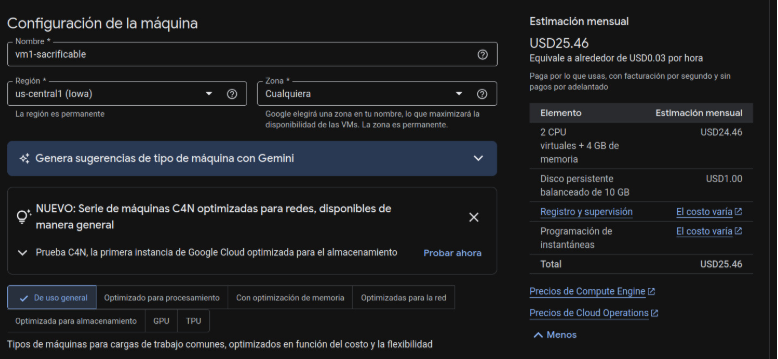
\includegraphics[width=0.95\textwidth]{figuras/metodologia/vm1_sacrificable.png}
  \caption{Configuración mostrada para la VM de control \texttt{vm1-sacrificable}.}
  \label{fig:vm1-configuracion}
\end{figure}

\begin{figure}[H]
  \centering
  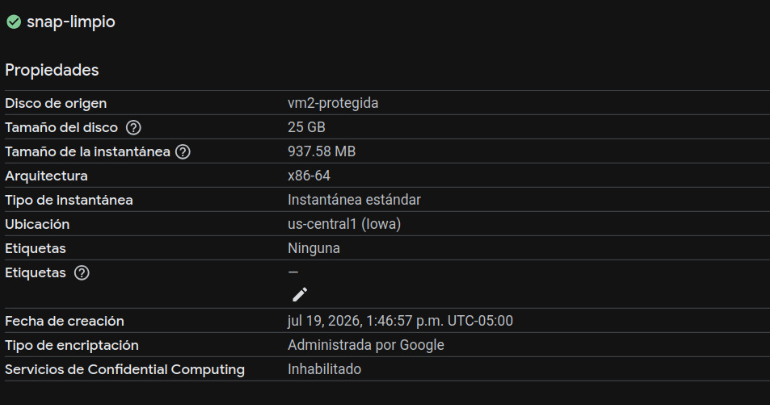
\includegraphics[width=0.95\textwidth]{figuras/metodologia/vm2_protegida_snapshot.png}
  \caption{Propiedades del snapshot \texttt{snap-limpio} asociado a \texttt{vm2-protegida}.}
  \label{fig:vm2-snapshot}
\end{figure}

Los campos no consignados en la Tabla~\ref{tab:entorno-evaluacion} no se
infirieron a partir de las Figuras~\ref{fig:vm1-configuracion} y
\ref{fig:vm2-snapshot}. Deben registrarse con
\texttt{scripts/validacion/preparar\_corrida.sh} antes de las repeticiones
finales. El diseño contempla tres repeticiones por condición. La evidencia
disponible en este informe es preliminar: incluye dos corridas sin protección
y una corrida con el monitor activo.

Los escenarios evaluables son línea base, proliferación de procesos, consumo
gradual de memoria y crecimiento de archivo. Para la comparación principal se
usa la misma carga de procesos en las VM de control y protegida. Los
simuladores de memoria y archivo se ejecutan por separado para evitar que sus
efectos se mezclen.

\section{Métricas}

Las métricas se obtienen de las capturas del recolector, el log JSON del
monitor, \texttt{/proc}, \texttt{free} y la salida del sistema. El instante de
inicio de la carga se denota por $t_0$; los tiempos de alerta y recuperación se
expresan respecto a ese instante.

\begin{table}[H]
  \centering
  \caption{Métricas y criterios de cálculo.}
  \label{tab:metricas-evaluacion}
  \small
  \begin{tabular}{p{0.25\textwidth}p{0.44\textwidth}p{0.20\textwidth}}
    \toprule
    Métrica & Cálculo & Fuente y unidad \\
    \midrule
    Alerta inicial & $t_{\mathrm{sospechosa}}-t_0$ & Log, segundos \\
    Alerta crítica & $t_{\mathrm{critica}}-t_0$ & Log, segundos \\
    Escalamiento & $t_{\mathrm{critica}}-t_{\mathrm{sospechosa}}$ & Log, segundos \\
    Pico de procesos & Máximo de procesos simultáneos & Recolector, procesos \\
    Procesos normalizados & $100N_{\mathrm{proc}}/N_{\mathrm{limite}}$ & Porcentaje \\
    Uso de RAM & $100M_{usada}/M_{asignada}$ & \texttt{free}, porcentaje \\
    Uso de CPU & Uso agregado dividido entre las vCPU asignadas & Porcentaje \\
    Recuperación & $t_{\mathrm{estable}}-t_{\mathrm{fin}}$ & Recolector, segundos \\
    Falsos positivos & Alertas críticas durante la línea base & Log, conteo \\
    Sobrecarga & Diferencia de CPU y RSS con y sin monitor & Porcentaje y MiB \\
    \bottomrule
  \end{tabular}
\end{table}

La mediana de las tres repeticiones será el valor representativo; el mínimo y
el máximo mostrarán la dispersión. Mientras no existan las tres corridas, se
reportan valores individuales y se identifican como preliminares. Los eventos
JSON se agrupan por marca temporal, severidad, PID y PGID. Una transición del
mismo PID desde \texttt{sospechosa} a \texttt{critica} representa persistencia,
no dos procesos diferentes.

\section{Procedimiento y medidas de seguridad}

Cada corrida sigue el mismo procedimiento:

\begin{enumerate}
  \item Restaurar el snapshot de la VM y comprobar RAM, vCPU, límite de PID,
        kernel y commit.
  \item Ejecutar \texttt{make check}, limpiar los logs de la corrida anterior
        e iniciar el recolector del sistema.
  \item Medir la línea base, registrar $t_0$ e iniciar una sola carga.
  \item En la VM protegida, iniciar primero Anti-Bunny Virus y comprobar el
        modo de respuesta, el usuario y el PGID autorizado.
  \item Registrar procesos, CPU, RAM, severidad, PID, PPID, PGID, ciclos y
        acciones hasta finalizar la carga y observar la recuperación.
  \item Copiar capturas y logs sin modificarlos, restaurar la VM y repetir el
        escenario tres veces.
\end{enumerate}

Las pruebas se limitan a VM aisladas, con consola disponible y usuario de
laboratorio sin privilegios. La unidad protegida aplica
\texttt{PIDsMax=256} como freno independiente. La contención solo puede
habilitarse en modo \texttt{terminar\_lab}, para un PGID publicado y un usuario
autorizado; en los demás casos el sistema únicamente alerta. No deben
ejecutarse cargas ilimitadas en el equipo anfitrión. Si la VM deja de responder,
se detiene la corrida desde el hipervisor y se restaura el snapshot.

El análisis conserva por separado los datos crudos y los datos derivados. El
archivo \texttt{informe/datos/anti\_bunny\_virus\_logs.json} es la fuente de la
tabla y la gráfica del sistema protegido; así se mantiene la trazabilidad entre
cada resultado y el evento original.

\chapter{Resultados y análisis}

\section{Verificación del sistema}

La ejecución de \texttt{make check} finalizó correctamente sobre la versión
integrada desde \texttt{main}. Se compilaron el monitor y los tres simuladores.
\texttt{tests/test\_motor\_deteccion} validó persistencia, escalamiento a
crítica y correlación de archivos; \texttt{tests/test\_respuesta} comprobó que
el modo \texttt{alerta} no envía señales y que \texttt{terminar\_lab} rechaza
alertas no críticas, PID~1, PGID inválidos, PGID no autorizado, UID incorrecto e
identidad obsoleta (\texttt{starttime}). También se validó la sintaxis de los
scripts y la política estática de contención en \texttt{respuesta.c}. Esta
verificación confirma el funcionamiento esperado del código refactorizado, pero
no sustituye las mediciones experimentales en las VM.

Las capturas registraron líneas base de 106 y 104 procesos, con 24,28\% y
23,86\% de RAM, respectivamente. No se dispone de una corrida independiente de
actividad normal con el monitor activo; por ello, no se calcula una tasa de
falsos positivos ni la sobrecarga del monitor.

\section{Funcionamiento ante proliferación de procesos}

\subsection{Prueba 1: carga moderada}

La primera corrida permitió observar la degradación inicial de la máquina
virtual durante la proliferación de procesos. La configuración y el estado
previo a la ejecución se muestran en la Figura~\ref{fig:fork-p1-inicio}. El
recolector tomó 55 muestras, con una línea base de 106 procesos y un máximo de
236. Durante la prueba, el uso máximo de CPU alcanzó 57,14\% y la RAM aumentó
de 24,28\% a 37,77\%, como resume la
Figura~\ref{fig:fork-p1-resultados}. Esta corrida muestra una carga moderada:
el número de procesos y el consumo de recursos aumentaron, pero no alcanzaron
la severidad observada en la segunda prueba.

\begin{figure}[H]
  \centering
  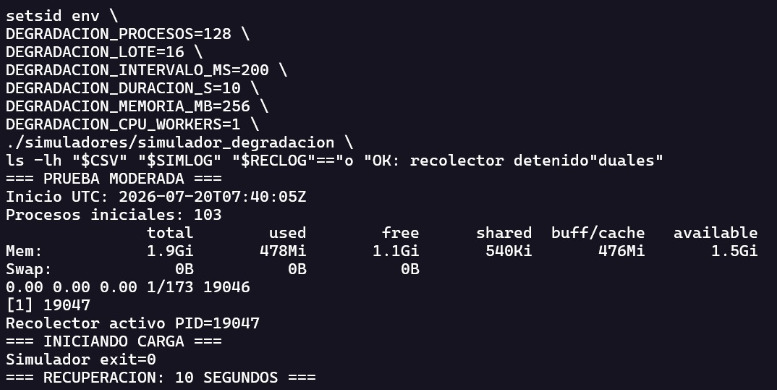
\includegraphics[width=0.94\textwidth]{figuras/anexos/fork_prueba_1_inicio.png}
  \caption{Prueba 1: configuración, línea base e inicio de la carga moderada.}
  \label{fig:fork-p1-inicio}
\end{figure}

\begin{figure}[H]
  \centering
  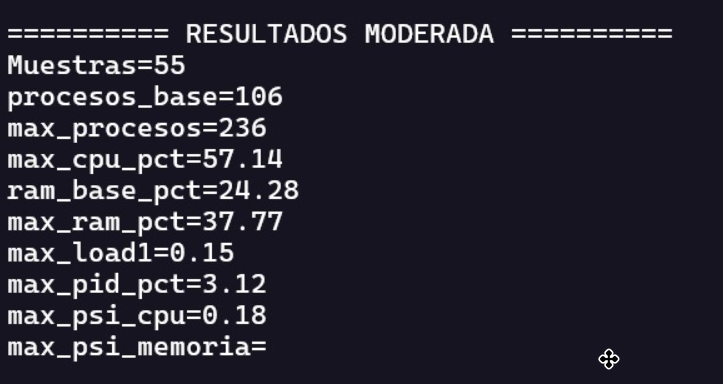
\includegraphics[width=0.94\textwidth]{figuras/anexos/fork_prueba_1_resultados.png}
  \caption{Prueba 1: resumen de mediciones de la carga moderada.}
  \label{fig:fork-p1-resultados}
\end{figure}

\subsection{Prueba 2: carga crítica}

La segunda corrida con fork bomb quedó incorporada al informe como evidencia
de carga crítica. La captura inicial registró 101 procesos
(Figura~\ref{fig:fork-p2-inicio}); el resumen del recolector reportó una línea
base de 104, un máximo de 619 procesos, CPU máxima de 100\% y uso máximo de RAM
de 73\% (Figura~\ref{fig:fork-p2-resultados}). Una captura adicional mostró 616
procesos y 1,4 GiB de memoria usada sobre 1,9 GiB disponibles en la máquina
virtual (Figura~\ref{fig:fork-p2-estado}). Estas observaciones corresponden a
una corrida y se conservarán como evidencia preliminar hasta completar las
repeticiones del protocolo.

\subsection{Evidencia con Anti-Bunny Virus activo}

La Figura~\ref{fig:sistema-anti-activo} muestra la salida del monitor durante
la carga de procesos. El archivo JSON asociado contiene 14 alertas de tipo
\texttt{procesos}, correspondientes a siete PID distintos del usuario
\texttt{antibunny-test}. Todos pertenecen al PGID 12480 y se ejecutaron en modo
\texttt{alerta}; por tanto, esta corrida permite evaluar la detección, pero no
la contención mediante señales.

\begin{figure}[H]
  \centering
  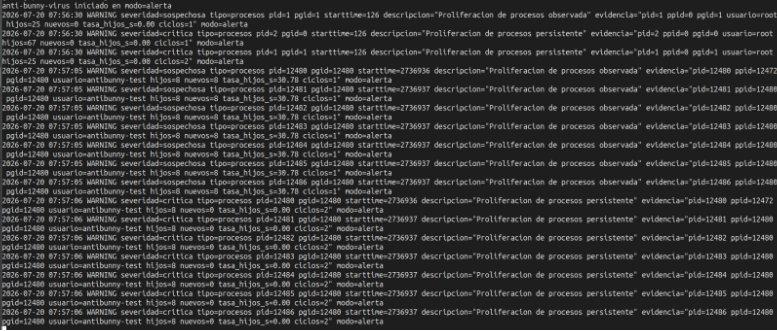
\includegraphics[width=\textwidth]{figuras/resultados/sistema_anti.png}
  \caption{Registro de Anti-Bunny Virus durante la detección de proliferación de procesos.}
  \label{fig:sistema-anti-activo}
\end{figure}

\begin{table}[H]
  \centering
  \caption{Resumen de eventos obtenidos del log JSON del sistema protegido.}
  \label{tab:eventos-antibunny}
  \small
  \begin{tabular}{p{0.43\textwidth}p{0.42\textwidth}}
    \toprule
    Indicador & Valor observado \\
    \midrule
    Intervalo registrado & 20-07-2026, 07:57:05--07:57:06 \\
    Eventos totales & 14 alertas \texttt{WARNING} \\
    Procesos distintos & 7 PID \\
    Grupo y usuario & PGID 12480; \texttt{antibunny-test} \\
    Primer ciclo & 7 alertas sospechosas; 8 hijos nuevos por PID \\
    Tasa máxima observada & 30,78 hijos/s \\
    Segundo ciclo & 7 alertas críticas por persistencia \\
    Modo de respuesta & \texttt{alerta}; sin terminación registrada \\
    \bottomrule
  \end{tabular}
\end{table}

La Figura~\ref{fig:evolucion-hijos-json} muestra la evolución por proceso que
puede reconstruirse del JSON. En el primer ciclo, cada uno de los siete PID
tenía ocho hijos y había creado ocho hijos nuevos, con una tasa máxima de 30,78
hijos/s; el sistema emitió una alerta sospechosa. En el segundo ciclo se
mantuvieron los ocho hijos, no aparecieron hijos nuevos y la persistencia elevó
la alerta a crítica. La caída de hijos nuevos a cero no demuestra que
Anti-Bunny Virus detuviera la carga: el log conserva ocho hijos por PID y fue
generado en modo \texttt{alerta}, sin señales de terminación.

\begin{figure}[H]
  \centering
  \begin{tikzpicture}
    \begin{axis}[
      ybar=2pt,
      width=0.88\textwidth,
      height=0.43\textwidth,
      bar width=24pt,
      ymin=0,
      ymax=9,
      ytick={0,1,...,9},
      xtick={1,2},
      xticklabels={Ciclo 1: sospechosa,Ciclo 2: crítica},
      xlabel={Ciclo de persistencia},
      ylabel={Hijos por proceso alertado},
      legend style={at={(0.5,1.02)},anchor=south,legend columns=2},
      grid=major,
      nodes near coords,
      enlarge x limits=0.35
    ]
      \addplot table[x=ciclo,y=hijos_por_pid,col sep=comma]
        {datos/anti_bunny_hijos_por_ciclo.csv};
      \addplot table[x=ciclo,y=nuevos_por_pid,col sep=comma]
        {datos/anti_bunny_hijos_por_ciclo.csv};
      \legend{Hijos presentes,Hijos nuevos}
    \end{axis}
  \end{tikzpicture}
  \caption{Evolución de hijos por proceso y escalamiento de la detección según el log JSON.}
  \label{fig:evolucion-hijos-json}
\end{figure}

\section{Comparación e interpretación}

La Tabla~\ref{tab:comparacion-resultados} resume las dos corridas sin protección
y la corrida con detección activa. El JSON protegido no registra procesos
totales, CPU ni RAM global.

\begin{table}[H]
  \centering
  \caption{Resumen de las corridas documentadas.}
  \label{tab:comparacion-resultados}
  \small
  \begin{tabular}{p{0.25\textwidth}p{0.20\textwidth}p{0.20\textwidth}p{0.22\textwidth}}
    \toprule
    Indicador & Prueba 1 & Prueba 2 & Anti-Bunny activo \\
    \midrule
    Condición & Sin monitor & Sin monitor & Modo \texttt{alerta} \\
    Procesos base & 106 & 104 & No registrado \\
    Máximo de procesos & 236 & 619 & No registrado \\
    Incremento respecto a base & 122,64\% & 495,19\% & No calculable \\
    CPU máxima & 57,14\% & 100\% & No registrada \\
    RAM inicial--máxima & 24,28--37,77\% & 23,86--73\% & No registrada \\
    Evidencia de detección & No aplica & No aplica & 7 sospechosas y 7 críticas \\
    Evidencia de contención & No aplica & No aplica & No; modo \texttt{alerta} \\
    \bottomrule
  \end{tabular}
\end{table}

\begin{itemize}
  \item Prueba 1: aumento de 130 procesos y 13,49 puntos porcentuales de RAM.
  \item Prueba 2: aumento de 515 procesos, CPU máxima de 100\% y aumento de
        49,14 puntos porcentuales de RAM.
  \item Anti-Bunny activo: siete PID pasaron de sospechosos a críticos en dos
        ciclos, con una tasa máxima de 30,78 hijos/s. No hubo contención porque
        el sistema operó en modo \texttt{alerta}.
\end{itemize}

\section{Hipótesis y limitaciones}

\textbf{Resultado de la hipótesis:} respaldo parcial. Se verificaron la
detección de procesos, el escalamiento por persistencia y los rechazos de
seguridad automatizados.

\textbf{Limitaciones:}
\begin{itemize}
  \item Dos corridas sin protección y una con detección; sin tres repeticiones
        equivalentes.
  \item Sin mediciones experimentales de memoria, archivos, falsos positivos,
        sobrecarga, contención o recuperación.
  \item Resultados limitados al entorno de VM y sin validación frente a malware
        real.
\end{itemize}

\chapter{Conclusiones}

\begin{enumerate}
  \item Sin protección, la corrida crítica alcanzó 619 procesos, 100\% de CPU
        y 73\% de RAM.
  \item Anti-Bunny Virus detectó siete PID y escaló sus alertas de sospechosas
        a críticas tras dos ciclos, con un máximo de 30,78 hijos/s.
  \item Las pruebas automatizadas confirmaron el rechazo de objetivos no
        autorizados y de identidades inválidas.
  \item La hipótesis quedó parcialmente respaldada: se validó la detección,
        pero no la contención experimental, la recuperación ni la sobrecarga.
\end{enumerate}

\section{Cumplimiento de objetivos}

\begin{table}[H]
  \centering
  \caption{Cumplimiento de los objetivos del proyecto.}
  \label{tab:cumplimiento-objetivos}
  \small
  \begin{tabular}{p{0.13\textwidth}p{0.18\textwidth}p{0.57\textwidth}}
    \toprule
    Objetivo & Estado & Evidencia \\
    \midrule
    General & Parcial & Prototipo implementado y detección de procesos demostrada; faltan pruebas experimentales de memoria, archivos y contención. \\
    OE1 & Parcial & El sistema recolecta PID, PPID, PGID, CPU, RSS y archivos; la evidencia entregada solo valida procesos. \\
    OE2 & Parcial & Siete PID escalaron de sospechosos a críticos tras dos ciclos, con máximo de 30,78 hijos/s. \\
    OE3 & Parcial & Las pruebas automatizadas validaron los rechazos de seguridad; no se registró terminación real de un PGID autorizado. \\
    OE4 & Parcial & Se documentaron dos corridas sin monitor y una con detección; faltan condiciones equivalentes, tres repeticiones, contención y sobrecarga. \\
    \bottomrule
  \end{tabular}
\end{table}


\bibliographystyle{IEEEtran}
\bibliography{referencias}

\appendix
% Se conserva únicamente el apéndice B solicitado.
\setcounter{chapter}{1}
\chapter{Logs y datos complementarios}

\section{Evidencia de pruebas con fork bomb}

La primera prueba se presenta directamente en el capítulo de resultados. Este
anexo conserva la salida original de la segunda corrida como evidencia
complementaria de la carga crítica.

Las capturas se presentan en el orden entregado: inicio de la corrida crítica,
resumen de resultados y estado observado con 616 procesos.

\begin{figure}[H]
  \centering
  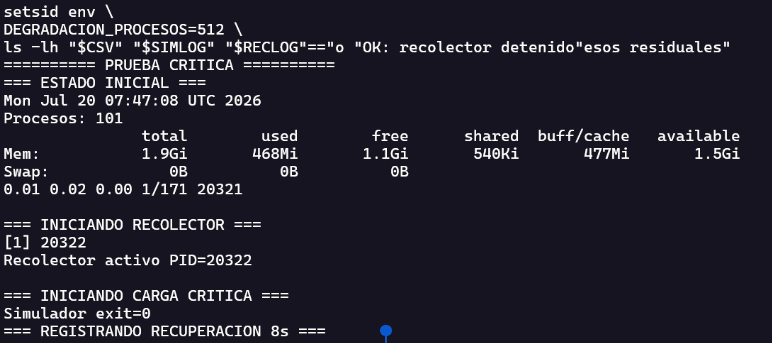
\includegraphics[width=0.94\textwidth]{figuras/anexos/fork_prueba_2_inicio.png}
  \caption{Prueba 2: estado inicial, inicio del recolector y ejecución de la carga crítica.}
  \label{fig:fork-p2-inicio}
\end{figure}

\begin{figure}[H]
  \centering
  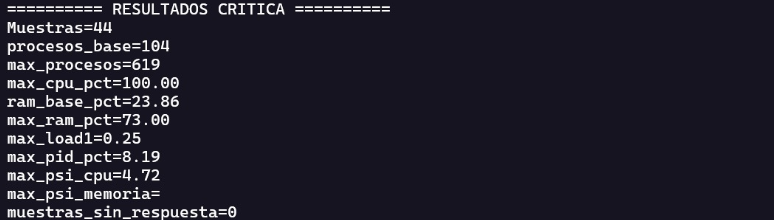
\includegraphics[width=0.94\textwidth]{figuras/anexos/fork_prueba_2_resultados.png}
  \caption{Prueba 2: resumen de mediciones de la carga crítica.}
  \label{fig:fork-p2-resultados}
\end{figure}

\begin{figure}[H]
  \centering
  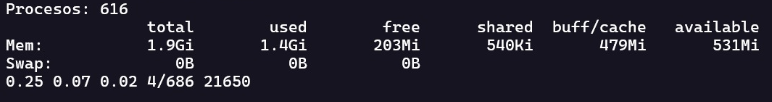
\includegraphics[width=0.94\textwidth]{figuras/anexos/fork_prueba_2_estado.png}
  \caption{Prueba 2: estado observado con 616 procesos y uso de memoria de la máquina virtual.}
  \label{fig:fork-p2-estado}
\end{figure}


\end{document}
